\chapter{Literature Review / Background}
\label{chap2}

To achieve reach our goal, we aim to construct a complex system that consists of multiple modules based on various fields of knowledge. This paragraph provides the key foundations upon which this thesis is built.

%==================================================
%==================================================
%==================================================
\section{Business Location Recommendation}

The optimal selection of business locations is a factor that significantly influences the success and sustainability of any enterprise. The placement of a business determines various other parameters, such as customer accessibility, operational efficiency, and
its overall profit in general. Prior studies \cite{paper_xorotaxias} have emphasized that optimal location selection not only can reduce urban shrinkage, but also strengthen the resilience of cities. These benefits of choosing the appropriate location, combined with its irreversible nature once performed, motivated the exploration of state-of-the-art technologies that may help address the problem. 

One field that has been increasingly utilized in recent years is Geographic Information Systems (GIS). As shown in prior work \cite{restaurant_rec_system}, spatial and GIS data enhance the location selection with important criteria, such as foot traffic, demographic patterns, and competitor distribution. The rapid increase of available data served as a catalyst for the evolution of machine learning to evolve. This application of artificial intelligence enables systems to automatically capture complex underlying patterns of data to make predictions in the future \cite{megacities_paper}. In recent years, groundbreaking approaches like Deep Learning, Transformers, and Large Language Models (LLMs) propose effective approaches to utilizing GIS data for optimal business location determination. Although limited research has been conducted on this topic, certain studies \cite{gpt_chatbots} \cite{llm_recommend_systems} suggest that LLMs can enhance the performance of location-based recommendation systems. 

Building upon these foundations, the following paragraphs dive deeper in GIS data in location analysis, multiple LLM-based systems (fine-tuned LLMs, RAG) and AI explainability while also examining the NACE business classification protocol.


%==================================================
%==================================================
%==================================================
\section{Geospatial Data and GIS in Location Analysis}

A Geographic Information System (GIS) is a system designed
to store, analyze, edit, and visualize geographic data \cite{Data_science_GIS}. It merges various types of data into a common framework, allowing users to capture and understand patterns, trends, and relationships in a spatial context. GIS data emerged in the early 1960s and initially focused on applications like map digitization and the conceptualization of spatial databases \cite{Data_science_GIS}. 

Since then, GIS has evolved into a versatile tool for spatial analysis, driven by breakthroughs in remote sensing data, both in terms of collection (e.g. satellite imagery, maps, demographic information), and accessibility (e.g. rise of location-based services, use of smartphones for real-time data collection). Certain fields that GIS data has been applied across include urban and infrastructure planning \cite{Data_science_GIS}, environmental analysis and conservation \cite{Data_science_GIS}, public health \cite{Epidemiologic_Studies}, enhancement of virtual assistants \cite{virtual_assistants}, public transportation accessibility and optimization \cite{public_transport_metropolitan}, and, of particular relevance to this thesis, business intelligence \cite{satelite_gis}. Within business location analysis in particular, GIS enables the integration of spatial factors such as population density, transportation accessibility, and competitor distribution \cite{gis_business_intelligence_e3s}. In addition, a rich ecosystem has been built around geospatial data, including a range of software platforms. In this thesis, QGIS, a powerful and open-source GIS software used for editing and visualizing geospatial data \cite{QGIS}, was employed to extract and process valuable geographical information in order to enhance our datasets. 

While Geographic Information Systems provide useful and interpretable tools, they mainly rely on static, rule-based algorithms that often fail to capture complex patterns. To address these limitations, machine learning frameworks have been increasingly integrated with GIS data, as discussed in the following sections.


%==================================================
%==================================================
%==================================================
\section{Machine Learning in Business Location Analysis}

Machine learning (ML) is a groundbreaking scientific field that focuses on the creation of models that are able to capture complex, non-linear underlying relationships, without the need to be explicitly programmed \cite{murphy2012ml}. The learning process is driven by data, based on which the model adapts to a specific application domain. In the context of this thesis, machine learning models are integrated with GIS data to augment business location analysis, particularly by incorporating features such as geographic coordinates (latitude and longitude), distance to the city center, proximity to transportation stations, and accessibility to key facilities such as the university or the port. Despite the importance of these models, we do not use them directly to generate the final recommendations. Rather, we apply ML as a supporting tool for building proxy ground truths and providing interpretability about the importance of the features. The actual predictions are produced by LLM-driven pipelines, which we explain later.


%==================================================
%==================================================
\subsection{Categories of Machine Learning}
The field of machine learning is divided into certain categories, determined by the labeling of the training dataset. 


\begin{itemize}
    \item \textbf{Supervised ML}: These algorithms learn by using labeled examples to predict future events from unseen data \cite{megacities_paper}. Although there is a variety of traditional and reliable supervised ML models, in this work we use certain state-of-the-art tree-based methods. Specifically, Random Forest is an ensemble-based method which combines multiple decision trees using bagging \cite{random_forest_breiman2001}, and XGBoost, a gradient boosting algorithm that sequentially builds ensembles of trees to minimize prediction error \cite{xgboost_chen2016}.

    \item \textbf{Unsupervised ML}: When labels are not available, unsupervised techniques are used discover underlying patterns within the dataset. In this thesis, K-Means clustering \cite{Kmeans_Ikotun2023} was applied to group neighborhoods into sets with similar characteristics. 

    \item \textbf{Semi-supervised ML}: In the course of this thesis, we frequently encountered the phenomenon of obtaining labels for only a small proportion of the data. Semi-supervised methods, such as Self-Training, aim to exploit limited labels to predict the missing ones, thus enhriching the dataset \cite{Rosidi2024SemiSupervised}.
\end{itemize}



%==================================================
%==================================================
\subsection{Explainable AI and SHAP}

Modern ML models manage to capture non-linear underlying patterns that rule-based algorithms cannot detect. However, applying complex models comes with the cost of failing to understand their decision-making, as they often act as black boxes. In order to identify the features that affect the model output, Explainable AI (XAI) techniques have been developed to unravel some of these aspects.

SHAP is a prominent XAI method based on cooperative game theory, used to increase the transparency and interpretability of machine learning models \cite{SHAP_Trevisan2022}. It provides insights into the importance of every feature by assigning a value that represents its contribution to a specific prediction. Within this thesis in particular, we calculate the SHAP values of every feature per NACE code, in order to determine the most impactful factors for every business type. The most important features of the location are then included as justifications during the creation of the fine-tuning dataset, as we will see below. 
 

%==================================================
%==================================================
%==================================================
\section{NACE Codes and Economic Classification}

NACE is the European standard classification of productive economic activities \cite{nace2008}. Providing a standardized categorization protocol is crucial for ensuring consistency across regions and time. Eurostat uses NACE to perform statistical reporting, as consistent classification enables better storing, processing, and merging heterogeneous data sources across different countries. The protocol follows a 4-level hierarchical structure, with business categorization getting increasingly detailed as the code gains precision. Specifically, the NACE code levels are the following: 

\begin{itemize} 
    \item \textbf{Sections}: first level, identified by an alphabetical code 
    \item \textbf{Divisions}: second level, identified by a two-digit numerical code 
    \item \textbf{Groups}: third level, identified by a three-digit numerical code 
    \item \textbf{Class}: fourth level, identified by a four-digit numerical code 
\end{itemize}

\noindent For instance, the retail sale of clothing uses the following classification values per level:

\begin{itemize}
    \item \textbf{Section G}: Wholesale and retail trade; repair of motor vehicles and motorcycles
    \item \textbf{Division 47}: Retail trade, except of motor vehicles and motorcycles
    \item \textbf{Group 47.7}: Retail sale of other goods in specialized stores
    \item \textbf{Class 47.71}: Retail sale of clothing in specialized stores
\end{itemize}

In the context of this thesis, we aim to collect multiple records of business activities in Volos. NACE will be used to effectively classify those enterprises and identify the ideal locations for each category. This thesis uses NACE Rev. 2, the current standard adopted in 2008.



%==================================================
%==================================================
%==================================================
\section{LLMs and Fine-Tuning Techniques}
\label{sec:lit_ft}

Although traditional ML models have been integrated into recommendation systems, nowadays the focus has shifted to the new architecture of Large Language Models (LLMs). Below, we first provide the foundations of LLMs and then examine how they can be adapted to a specific field, such as location-based recommendation.


%==================================================
%==================================================
\subsection{Introduction to Transformers \& LLMs}


Transformers are a groundbreaking machine learning technology that combines the methods of deep learning with the attention mechanism. Inspired by the 2017 paper ”Attention Is All You Need” \cite{attention_paper}, the attention mechanism is a method that enhances the vector representation of every text component with context information. In recent years, transformers have emerged as the state-of-the-art technology in machine learning, serving as the backbone of Large Language Models. Large Language Models (LLMs) are NLP models trained on extensive textual data that exhibit unparalleled
understanding of natural language patterns \cite{llm_recommend_systems}. Their ability to provide context-aware and personalized suggestions shows potential to improve recommendation systems. Multiple attempts have already been made to integrate LLMs in recommendation systems, such as GPT-based ChatBots that utilize ChatGPT \cite{gpt_chatbots}. Since general-purpose LLMs are trained on a broad web corpora, they are not specialized in an individual field. To achieve domain-specific knowledge, various adaptation techniques such as fine-tuning are applied. 


%==================================================
%==================================================
\subsection{Fine-Tuning Approaches}

The motivation of this thesis is our desire to use an LLM-based approach in a specific task (business location recommendation). Training an LLM from scratch is computationally infeasible in practice, as it adapts billions of parameters and requires extensively large datasets and computational resources. The most frequent approach involves adapting an existing pre-trained model by modifying its parameters, based on domain-specific data \cite{ft_Howard2018ULMFiT}. This technique is called LLM fine-tuning, and has multiple variations which we analyze below.


%==================================================
%==================================================
\subsubsection{Full-Model Fine-Tuning}

Full-model fine-tuning focuses on updating the entire set of model weights to fit the specific task. While this approach can provide the maximum adaptability to the target domain, it remains resource-intensive and is generally impractical for simple research projects \cite{pre_ft_ElKhoury2024LLMRecsys}. In order to make the LLM adaptation feasible, several techniques that perform fine-tuning more efficiently have been developed.


%==================================================
%==================================================
\subsubsection{Parameter-Efficient Fine-Tuning (PEFT)}


Parameter-efficient fine-tuning (PEFT) involves updating a relatively small proportion of the parameters while keeping the majority of the model frozen, in order to reduce computational cost and avoid overfitting. This approach drastically reduces the training parameters while retaining the general prior knowledge of the LLM.

\begin{figure}[h]
    \centering
    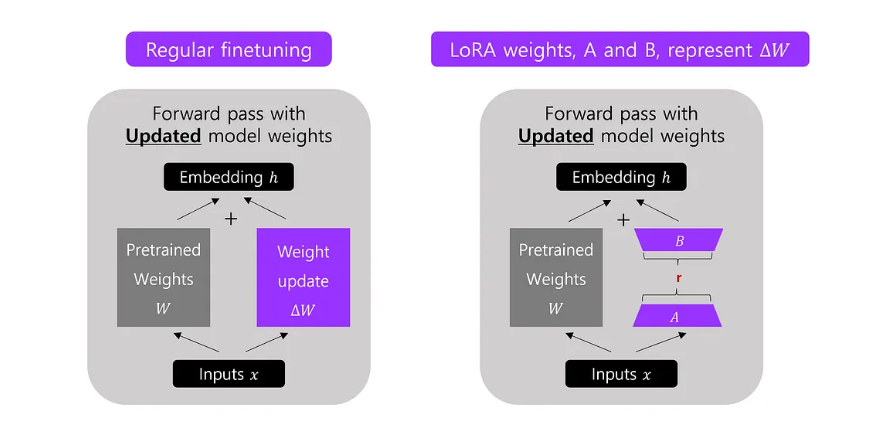
\includegraphics[width=0.8\textwidth]{figures/lora.png}
    \caption{Full Fine-Tuning Vs LoRA}
    \label{fig:lora}
\end{figure}


One popular emerging method that has been developed to achieve this goal is Low-Rank Adaptation (LoRA). This technique injects low-rank matrices into the weight matrices of the transformer layers \cite{pre_ft_ElKhoury2024LLMRecsys}, which serve as the only trainable parameters during fine-tuning. The small proportion of trainable weights enables efficient adaptation with minimal overhead, that both preserves the pre-trained knowledge of the model and adapts to the desired domain. Figure \ref{fig:lora} displays the difference between full fine-tuning and LoRA. An extension of LoRA, Quantized LoRA (QLoRA) further optimizes the fine-tuning process by quantizing the LLM in 4-bit precision. This significantly reduces the memory requirements for training, making it feasible to fine-tune LLMs on consumer-grade GPUs \cite{pre_ft_ElKhoury2024LLMRecsys}.


%==================================================
%==================================================
\subsection{Role in Thesis}

In the context of this thesis, the base model "mistralai/Mistral-7B-Instruct-v0.2" was fine-tuned using QLoRA. In order to lower the memory footprint, we applied 4-bit NF4 quantization and gradient checkpointing, which only stores a few “checkpoint” activations computed during the forward pass of model training. The LoRA configuration contained a rank of 16, a scaling factor of 64, that controls the magnitude of the LoRA update relative to the frozen base model, and a dropout rate of 0.05 to prevent overfitting. A more detailed explanation of the fine-tuned LLM system is presented in section \ref{sec:fine_tuned_llm}.

%==================================================
%==================================================
\subsection{Limitations}

While PEFT techniques significantly enable efficient fine-tuning, the approach of using a single model is prone to several disadvantages. Its main limitation resides in the static nature of the memory of the produced LLM. If we desire to update the knowledge of the model, we are forced to re-train it on updated data. Although the computational cost can be reduced by methods such as QLoRA, fine-tuning remains a time-consuming process we wish to avoid. The fine-tuned model can also suffer from hallucinations, as there is no guarantee that the generated output will always be accurate. To address these challenges, several alternative methods have been developed, such as  Retrieval-Augmented Generation, which we explain in detail below.



%==================================================
%==================================================
%==================================================
\section{Retrieval-Augmented Generation (RAG)}
\label{sec:lit_rag}

Fine-tuning an LLM to adapt to a specific task results in a specialized but relatively static model, prone to hallucinations. Retrieval-Augmented Generation (RAG) is a technique developed to solve these problems by leveraging dynamic knowledge.


%==================================================
%==================================================
\subsection{Introduction to RAG}

RAG is a method that enhances language model generation by incorporating external knowledge. Instead of relying on the memory stored in the model weights, we retrieve relevant information, typically documents or chunks of text, from external sources (e.g. files, databases), and feed it to the LLM to generate the final output \cite{RAG_Kumawat2024}. This approach enables dynamic memory updating, as the knowledge of the model is stored outside of the LLM and can be modified. In addition, it drastically reduces the hallucinations, as the information is retrieved in real time from the outer source and passed to the LLM. Figure \ref{fig:rag_concept} displays the workflow of a RAG system.

\begin{figure}[h]
    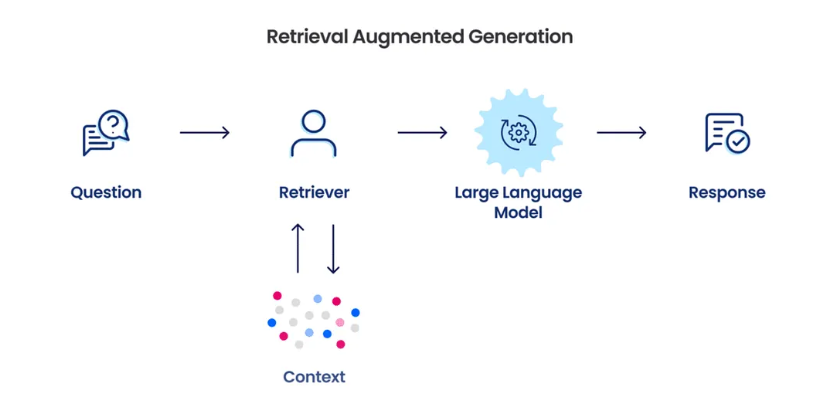
\includegraphics[scale=0.65]{figures/rag_concept.png}
    \centering
    \caption{Retrieval-Augmented Generation Workflow}
    \label{fig:rag_concept}
\end{figure}


%==================================================
%==================================================
\subsection{General RAG Workflow}

The general workflow of a RAG system usually involves two main steps: retrieval and generation, each corresponding to a component, the retriever and the generator, respectively. 

\begin{itemize}
    \item \textbf{Retriever:} Responsible for fetching  relevant information from external knowledge sources. It typically uses an embedder model, which encodes the user rquery in real time, and performs a similarity search with the pre-computed embeddings stored in the sources. The most relevant documents are selected and returned for the generation step.

    \item \textbf{Generator:} A generative Large Language Model that receives the retrieved information and generates a context-aware coherent output. By basing the generation on the retrieved data  the risk of hallucinations is mitigated.
\end{itemize}



%==================================================
%==================================================
\subsection{Role in Thesis}

Within this thesis, the retriever we use is "BAAI/bge-large-en-v1.5". This is a BERT-based encoder with 355 million parameters. The generator we select is "Llama 3" with 8 billion parameters. Before deploying the RAG framework, we apply the embedder on the neighborhood and NACE descriptions to pre-compute their vector representations, so we can simply load them during runtime. The process involves encoding the user query in real-time, performing a similarity search with the NACE embeddings to extract the desired business type, and another similarity search, this time with the neighborhood embeddings, to suggest recommendations that align with user preferences. The selected locations are then fed into the generator along with their descriptions to construct the final user output. A more detailed explanation of the RAG pipeline system is presented in section \ref{sec:rag}.




%==================================================
%==================================================
\subsection{Limitations}

Although utilizing a RAG pipeline addresses certain challenges presented in the fine-tuning approach, it introduces its own set of limitations. Since the pipeline consists of multiple modules, the inference time is bigger, making the system slower. In addition, the structure of the system largely depends on the quality of the retriever and the generator, chaining it to their own weaknesses. Finally, it usually requires additional infrastructure for storing the pre-computed embeddings. 


%==================================================
%==================================================
%==================================================
\section{Introduction to Chatbots}

Chatbots are advanced generative AI models that thrive at understanding and generating human language. Over the recent years, they have undergone a significant change in terms of quality and implementation, due to the emergence of Large Language Models (LLMs) \cite{chatbots_hundertmark2024}. While traditional chatbots used simple keyword-based rules to answer questions, modern chatbots  enhance user experience by leveraging the state-of-the-art NLP ability of LLMs, enabling dynamic request-response conversations with personalized and context-aware responses. This has motivated the application of chatbots to various domains in order to provide new insights and hopefully better accuracy and performance.

While regular LLMs receive a text input and return a text output, the consecutive queries are independent and lack the context of the conversation. A chatbot wraps around an LLM by adding features that essentially transform the LLM into a complete application. The two LLM-based approaches we described in sections \ref{sec:lit_ft} and \ref{sec:lit_rag} are the brain of the system. We will add features such as dialog and memory management, an interface layer, and communication between the frontend and backend components, in order to create a user-friendly chatbot application.

Since chatbots are built upon LLMs, they inherit not only their strengths, but their limitations as well. They are also even harder to evaluate, as their predictions depend on the conversation history.
In the context of this thesis, we aim to integrate a fine-tuned LLM approach and a RAG pipeline into a chatbot application, in order to exploit the advantages and disadvantages of each method.


%==================================================
%==================================================
%==================================================
\section{Summary}

In this chapter, we reviewed the research areas most relevant to the problem of business location recommendations, which form the basis of this thesis. We started by mentioning the motivation behind improving business location recommendation, and how GIS data enhance location analysis by providing geographic and demographic content. Next, we introduced machine learning and its integration with GIS, highlighting how ML models were used as supportive tools for generating proxy ground truths and providing interpretability. NACE codes were presented as a classification technique for economic activities. Moreover, we examined LLMs and domain-specific adaptation through fine-tuning, as well as the RAG framework and its components. Both approaches present different strengths and limitations, which we aim to exploit in the following chapters. Finally, we reviewed the process of transforming a simple LLM-based system into a chatbot application.
